\section{\hologo{hduthesis} 模板介绍}

\hologo{hduthesis}(\textbf Hangzhou \textbf Dianzi \textbf University \hologo{LaTeX} \textbf{Thesis} Template) 是杭州电子科技大学学位论文 \underline{非官方} \hologo{LaTeX} 模板,以 \hologo{LaTeX3} 构建,支持学士和硕士学位论文排版.

本模板文档将尽量完整地介绍模板的使用方法,如有不清楚之处,或者想提出改进建议,可以在 \href{https://github.com/myhsia/hduthesis/issues}{GitHub Issues} 提交反馈意见及贡献代码.

对于未接触过 \hologo{LaTeX} 的初学者,推荐阅读
\href{https://tug.ctan.org/info/lshort/english/lshort.pdf}
  {\emph{The Not So Short Introduction to \hologo{LaTeX2e}}}
(可在终端执行 \cmd{texdoc lshort} 获取)或者其中文版
\href{http://mirrors.ctan.org/info/lshort/chinese/lshort-zh-cn.pdf}
  {\emph{《一份(不太)简短的 \hologo{LaTeX2e} 介绍》}}
(可在终端执行 \cmd{texdoc lshort-zh-cn} 获取).

\subsection{模板组成}

\hologo{hduthesis} 模板的 \file{./tex/} 文件夹中包含了模板的所有 Runtime 文件.
其中,\file{hduthesis.cls} 是模板的核心文件,实质上并不提供主要功能,只用于对全局选项的控制加载模板的各个模块. 模板的功能模块如下

\begin{tasks}(2)
  \task! \file{typeset}:排版模块,用于控制字体和公式设置.
  \task! \file{layout}:版面模块,用于提供封面所用到的盒子和对输入文档信息的处理.
  \task \file{bc.config}:本科学位论文配置模块.
  \task \file{pg.config}:硕士学位论文配置模块.
  \task \file{hdu.l3doc}:用户手册模块.
  \task \file{hdu.stationery}:信纸模块.
\end{tasks}

以上模块包含在 \file{hduthesis-}\meta{模块名}\file{-module.code.tex} 文件中.
同时,\file{./tex/} 文件夹中还包含了 \file{hdulogo.pdf}、\file{hdutitle.pdf}、\file{hdumotto.pdf}、\file{hdubadge.pdf},分别提供杭州电子科技大学校徽、校名、校训和校牌的矢量图.
\footnote
  {
    这些矢量图均由 \href{https://www.hdu.edu.cn/666/list.htm}{校情纵览/校标规范} 所提供素材用 \href{https://inkscape.org}{Inkscape} 裁切制成. 如果你通过 \cmd{tlmgr} 安装了此模板,在其他文档类中也可以调用这些素材,并支持在 \hologo{XeLaTeX} 和 \hologo{pdfLaTeX} 编译器下使用 \cmd{Ti\textit k\/Z} 等方式设置透明度.
  }

模板预制的宏包有

\begin{table}[htbp]
  \centering \renewcommand* \arraystretch {.72}
  \begin{tabularx}{\linewidth}{*{9}{>{\footnotesize}X}}
    \toprule
    \pkg{amssymb}    & \pkg{bm}         & \pkg{booktabs}  &
    \pkg{cancel}     & \pkg{circuitikz} & \pkg{cleveref}  &
    \pkg{derivative} & \pkg{extarrows}  & \pkg{fixdif}   \\
    \midrule
    \pkg{hyperref}   & \pkg{listings}   & \pkg{mathtools} &
    \pkg{multicol}   & \pkg{pgfplots}   & \pkg{physics2}  &
    \pkg{siunitx}    & \multicolumn{2}{>{\footnotesize}l}{\pkg{unicode-math}}\\
    \bottomrule
  \end{tabularx}
\end{table}

\subsection{文件结构}

\subsubsection{用户手册}

\begin{center}
  \begin{minipage}{.36\linewidth}
    \dirtree
    {%
      .1 ./doc/.
      .2 hduthesis.tex.
      .2 hduthesis.pdf.
    }
  \end{minipage}
  \hfill
  \begin{minipage}{.6\linewidth}
    \dirtree
    {%
      .1 ./example/.
      .2 hduthesis-bc.tex, hduthesis-bc.pdf.
      .2 hduthesis-pg.tex, hduthesis-pg.pdf.
    }
  \end{minipage}
\end{center}

\subsubsection{Runtime 文件}

\dirtree
  {%
    .1 ./tex/.
    .2 hduthesis.cls.
    .2 hduthesis-typeset-module.code.
    .2 hduthesis-layout-module.code.
    .2 hduthesis-bc.config-module.code.
    .2 hduthesis-pg.config-module.code.
    .2 hduthesis-hdu.l3doc-module.code.
    .2 hduthesis-hdu.stationery-module.code.
    .2 hdulogo.pdf, hdutitle.pdf, hdumotto.pdf, hdubadge.pdf.
  }

\subsubsection{许可证}

\dirtree
  {%
    .1 ./LICENSE, README.md.
  }
\section{模板安装}

\subsection{系统要求}

本模板支持在 \cmd{macOS}、\cmd{Windows}、\cmd{Linux}、\cmd{Overleaf}、\cmd{TeXPage} 等平台使用.
\footnote
  {
    所使用的测试平台为 \cmd{macOS Sequoia Version 15.3}、\cmd{Ubuntu 24.04.1 LTS}、\cmd{Overleaf} 上的 \hologo{TeX} Live 2024 发行版,本模板均可顺利编译.
  }
本模板最低兼容发行版 \hologo{TeX} Live 2022,推荐使用 \hologo{TeX} Live 2023 或更新版本.
\footnote
  { 发行版 \hologo{TeX} Live 2022 中不包含 \pkg{physics2} 宏包,无法快捷输入等高括号. }
\footnote
  {
    发行版 \hologo{TeX} Live 2022 中通过导言区设置中文字体伪粗体和伪斜体时可能遇到报错. 详情请见 3.2 节.
  }
\footnote
  {
    根据 \emph{Plan for \hologo{TeX} Live 2025: 22feb: code freeze for final build, major bug fixes only; 1mar: final updates from CTAN, final doc tweaks.} 本模板将于 2025 年 2 月 22 日移除对 \hologo{TeX} Live 2022 的兼容,建议 \hologo{TeX} Live 2022 用户尽快升级至最新发行版.
  }
使用本模板生成学位论文,仅支持 \hologo{XeLaTeX} 编译;使用本模板生成信纸,支持 \hologo{pdfLaTeX} 编译.

\subsection{标准安装}

强烈建议您使用 \cmd{tlmgr} 进行安装与升级. 在终端(Terminal)执行以下命令即可安装最新版本的 \hologo{hduthesis} 模板.

\begin{framed}
  \begin{verbatim}
    sudo tlmgr install hduthesis
  \end{verbatim}
\end{framed}

Windows 系统用户无需 \verb|sudo|,请以管理员身份运行命令提示符. 有些时候,您需要手动更新 \cmd{tlmgr}

\begin{framed}
  \begin{verbatim}
    sudo tlmgr update --self
  \end{verbatim}
\end{framed}

才能正常使用 \cmd{tlmgr} 命令安装宏包.
如果您的 \hologo{TeX} 发行版不支持 \cmd{tlmgr},请尽快升级您的 \hologo{TeX} 发行版.
升级该模板,在终端(Terminal)执行以下命令即可

\begin{framed}
  \begin{verbatim}
    sudo tlmgr update hduthesis
  \end{verbatim}
\end{framed}

\subsection{手动安装}

本模板已上传至 CTAN、GitHub 和 Gitee 平台. 可以直接从三个平台下载最新版本的 \hologo{hduthesis} 模板. 下载后,将 \file{./hduthesis/tex/} 文件夹中的所有 (runtime) 文件复制到 \file{./hduthesis/example/} 目录下,即可编译 \file{./hduthesis/example/} 文件夹中的样例.

\section{全局选项}

\subsection{用户协议}

使用本模板编译本科、硕士学位论文时遇到``编译受阻''报错,请认真阅读封面的用户协议.
添加选项 \cmd{agreed} 后(即\verb|\documentclass [ agreed ] { hduthesis }|),方可顺利编译,\emph{并默认您已同意用户协议}.

使用 \hologo{hduthesis} 编译信纸和本用户手册时,无需 \cmd{agreed} 选项.

\subsection{字体设置}

用户可通过全局选项设置文档的数学和中文字体. 设置的方式为键值对,键 \keys{\cmdmac~math-font} 用于设置数学字体,键 \keys{\cmdmac~CJKmain-font} 用于设置中文字体,键 \keys{\cmdmac~CJKsans-font} 用于设置中文无衬线字体. 以下是设置示例.

\begin{framed}
  \begin{verbatim}
    \documentclass
      [
        math-font    = STIX Two Math, agreed,
        CJKmain-font = {{Songti SC}[AutoFakeBold = 2.5, AutoFakeSlant]},
        CJKsans-font = {{STHeiti}[AutoFakeBold = 2]}
      ] {hduthesis}
  \end{verbatim}
\end{framed}

如果你使用的是 \hologo{TeX} Live 2022,设置中文字体的伪粗体和伪斜体时可能会遇到报错.
在此发行版中,最多能对两个选项中的其一赋强度值,且被赋值选项需放在未被赋值选项前.

更加详细的字体设置请参考 \pkg{xeCJK} 宏包的文档.

\section{文档信息设置}

\begin{function}{\DocInfo}
  \begin{syntax}
    \cs{DocInfo}\marg{keyvals}
  \end{syntax}

  此命令接收键值,用于设置文档信息. 键 \keys{\cmdmac~title} 用于设置论文标题,键 \keys{\cmdmac~department} 用于设置学院,键 \keys{\cmdmac~major} 用于设置专业,键 \keys{\cmdmac~class} 用于设置班级,键 \keys{\cmdmac~stdntid} 用于设置学号,键 \keys{\cmdmac~author} 用于设置作者,键 \keys{\cmdmac~supervisor} 用于设置导师,键 \keys{\cmdmac~bibsource} 用于设置插入参考文献文件源. 命令会根据输入的学号自动判断使用者为本科生/研究生.

  命令 \cs{DocInfo} 需在导言区中执行. 完成文档信息输入后,在 \verb|\begin{document}| 后执行命令 \cs{maketitle} 会调用所设置的键值自动生成 \emph*{论文封面} 和 \emph*{目录}.
\end{function}

本科生输入样例如下. 需要使用键 \keys{\cmdmac~title} 设置类型为毕业设计/毕业论文,使用斜线 (/) 分隔,如 \cmd{title = 杭州电子科技大学学位论文 \hologo{LaTeX} 模板/毕业论文}.

\begin{framed}
  \begin{verbatim}
    \DocInfo
      {
        title  = 杭州电子科技大学学位论文 \hologo{LaTeX} 模板/
                 本科毕业设计, department = 理学院, major = 物理学,
        bibsource  = reference, class  = 英才班, stdntid = C668668E,
        author     = 申智能,    supervisor = 教授:葉芷晴, 
      }
  \end{verbatim}
\end{framed}

研究生输入样例如下. 硕士学位论文扉页需同时有英文版,因此需要在键 \keys{\cmdmac~title} \keys{\cmdmac~author} \keys{\cmdmac~supervisor} 中分别输入中文和英文信息,中英信息使用斜线 (\cmd/) 分隔,指导教师职称和姓名之间用半角冒号 (\cmd:) 分隔.

\begin{framed}
  \begin{verbatim}
    \documentclass { hduthesis }
    \DocInfo
      {
        title      = 杭州电子科技大学学位论文 \hologo{LaTeX} 模板/
                     \hologo{LaTeX} Template for Thesis at
                     Hangzhou Dianzi University,
        major      = 物理学,             stdntid    = 216686680,
        author     = 申智能/SAN Chi Nan, bibsource  = reference
        supervisor = 教授:葉芷晴/Prof.:YIP Tsz Ching,
      }
  \end{verbatim}
\end{framed}

\subsection{生成封面 \& 扉页}

在正文区域,使用命令 \cmd{maketitle} 即可生成论文封面和扉页. 生成的封面和扉页会根据所设置的文档信息自动生成.

\DescribeMacro{\l__hduthesis_grade_int}
封面上的论文完成日期和学生毕业年份会根据当前系统时间自动生成.
针对本科论文,如果当前月份在8月及以前,毕业年份会显示今年;如果当前月份在9月及以后,毕业年份会显示次年. 在 \cs{DocInfo} 后对整型 \cs{l__hduthesis_grade_int} 重新赋值可手动更改毕业年份.

\begin{syntax}
  \cs{ExplSyntaxOn} \cs{int_set:Nn} \cs{l__hduthesis_grade_int} \marg{Year} \cs{ExplSyntaxOff}
\end{syntax}

\subsection{生成承诺书}

\begin{function}{\commitment}
  \begin{syntax}
    \cs{commitment} \oarg{file1/yyyy-mm-dd, file2/yyyy-mm-dd, file3/yyyy-mm-dd}
  \end{syntax}

  此命令用于生成承诺书. 命令的可选参数接收数组,用于指定签名文件和输入签名的日期. 签名文件和签名的日期之间用 \cmd{/} 分隔,多组签名之间用 \cmd{,} 分隔. 签名文件接收 \file{.pdf} / \file{.png} / \file{.jpg} 等格式. 日期的输入格式为 \texttt{yyyy-mm-dd}.
\end{function}

对于本科生,只需要签署 ``\emph*{诚信承诺}'' 一组签名;对于研生,则需要签署 ``\emph*{原创性声明}''、``\emph*{(作者同意)学位论文使用授权声明}'' 和 ``\emph*{(导师同意)学位论文使用授权声明}'' 三组签名. 使用用例如下

\begin{framed}
  \begin{verbatim}
    % 本科生使用用例
    ... \maketitle ... \commitment [ example-image-a/2024-05-31 ] ...
    % 研究生使用用例
    ... \maketitle ...
    \commitment
      [
        example-image-a/2025-05-31, example-image-a/2025-05-31,
        example-image-b/2025-06-01
      ]
  \end{verbatim}
\end{framed}

如果使用者暂未生成签名但是需要添加日期,则将签名文件留空即可,但分隔符 \cmd{/} 仍需保留. 例如 
\verb|\commitment [ /2024-05-31 ]|. 如果不需要添加日期,则直接留空即可.

下两页分别为所生成的本科和硕士学位论文封面、扉页和承诺书缩略图. 可在终端执行 \cmd{texdoc hduthesis-bc} 和 \cmd{texdoc hduthesis-pg}  分别获取本科和硕士学位论文样例文件.

\includepdfmerge
  [ nup = 2x3, frame, linktodoc, scale = 0.96, delta = 1in .25in ]
  { /Users/myhsia/Documents/GitHub/hduthesis/example/hduthesis-bc.pdf, 1-2,
    /Users/myhsia/Documents/GitHub/hduthesis/example/hduthesis-pg.pdf, 1-4 }

\section{章节设置}

\subsection{输入中 / 英摘要}

\DescribeEnv{abstract}
环境 \env{abstract} 用于生成摘要,其可选参数可设置语言格式.

\DescribeMacro{\keywords}
命令 \cs{keywords} 需在 \env{abstract} 环境内执行,其会根据 \env{abstract} 环境所选择的语言,自动生成英文 / 中文格式的关键词.

\begin{framed}
  \begin{verbatim}
    \begin{abstract}[en]...\keywords{keyword1, keyword2}  \end{abstract}
    \begin{abstract}[cn]...\keywords{关键词1, 关键词2}   \end{abstract}
  \end{verbatim}
\end{framed}

通过命令 \cs{keywords} 以半角逗号 (,) 为分隔输入关键词列表,输出时会根据所处 \env{abstract} 环境选择的语言不同,自动以半 / 全角分号分隔.

\subsection{输入目录 \& 正文}

通过命令 \cs{tableofcontents} 可生成目录. \cs{chapter}、\cs{section}、\cs{subsection} 等章节级次均按照 \href{https://jwc.hdu.edu.cn/2022/0428/c4528a153813/page.htm}{杭电理工类毕业论文写作规范} 定制.

\subsection{参考文献 \& 附录}

通过命令 \cs{DocInfo} 指定 \file{.bib} 文件后使用命令 \cs{printbiblography} 即可输出参考文献列表. 参考文献格式已设置为 \cmd{gb7714-2015}. 若未指定参考文献 \file{.bib} 文件,为加速编译,\pkg{gbt7714} 宏包将不会加载.

可以直接使用带有星号的章节命令生成附录章节,如 \verb|\chapter*{附录}|.

\clearpage

\section{附加模块}

\subsection{杭州电子科技大学信纸}

加载全局选项 \pkg{stationery},并进行文档信息设置,即可生成信纸. 可用于推荐信撰写或生成笔记纸.
此模块无需 \pkg{agreed} 选项.

\begin{framed}
  \begin{verbatim}
    \documentclass [ stationery ] { hduthesis }
  \end{verbatim}
\end{framed}

与学士 / 硕士学位论文文档信息设置类似,使用 \cs{DocInfo} 命令,对信件主题、发件人、邮箱、日期和水印进行设置. 此时 \cs{DocInfo} 命令接受键
\keys{\cmdmac~title} \keys{\cmdmac~author} \keys{\cmdmac~mail}
\keys{\cmdmac~date} \keys{\cmdmac~watermark}. 下页为生成信纸的样例.

\begin{framed}
  \begin{verbatim}
    \DocInfo
      {
        title      = Recommendation Letter for SAN Chi Nan,
        author     = YIP Tsz Ching, mail = email@server.domain,
        date       = {23\textsuperscript{th} December, 2024},
        watermark  = true
      }
  \end{verbatim}
\end{framed}

若要在信纸上添加笔记线,可使用命令 \cs{noteLine}\oarg{num},其可选参数接收笔记线的数量,默认值为20. 下两页分别为生成的信纸和笔记纸样例,可在终端执行 \cmd{texdoc hduthesis-stationery} 获取此样例文件.

\subsection{用户手册}

本手册为 \cls{hduthesis} 加载选项 \pkg{l3doc} 后生成,此模块无需 \pkg{agreed} 选项.

\begin{framed}
  \begin{verbatim}
    \documentclass [ l3doc ] { hduthesis }
  \end{verbatim}
\end{framed}

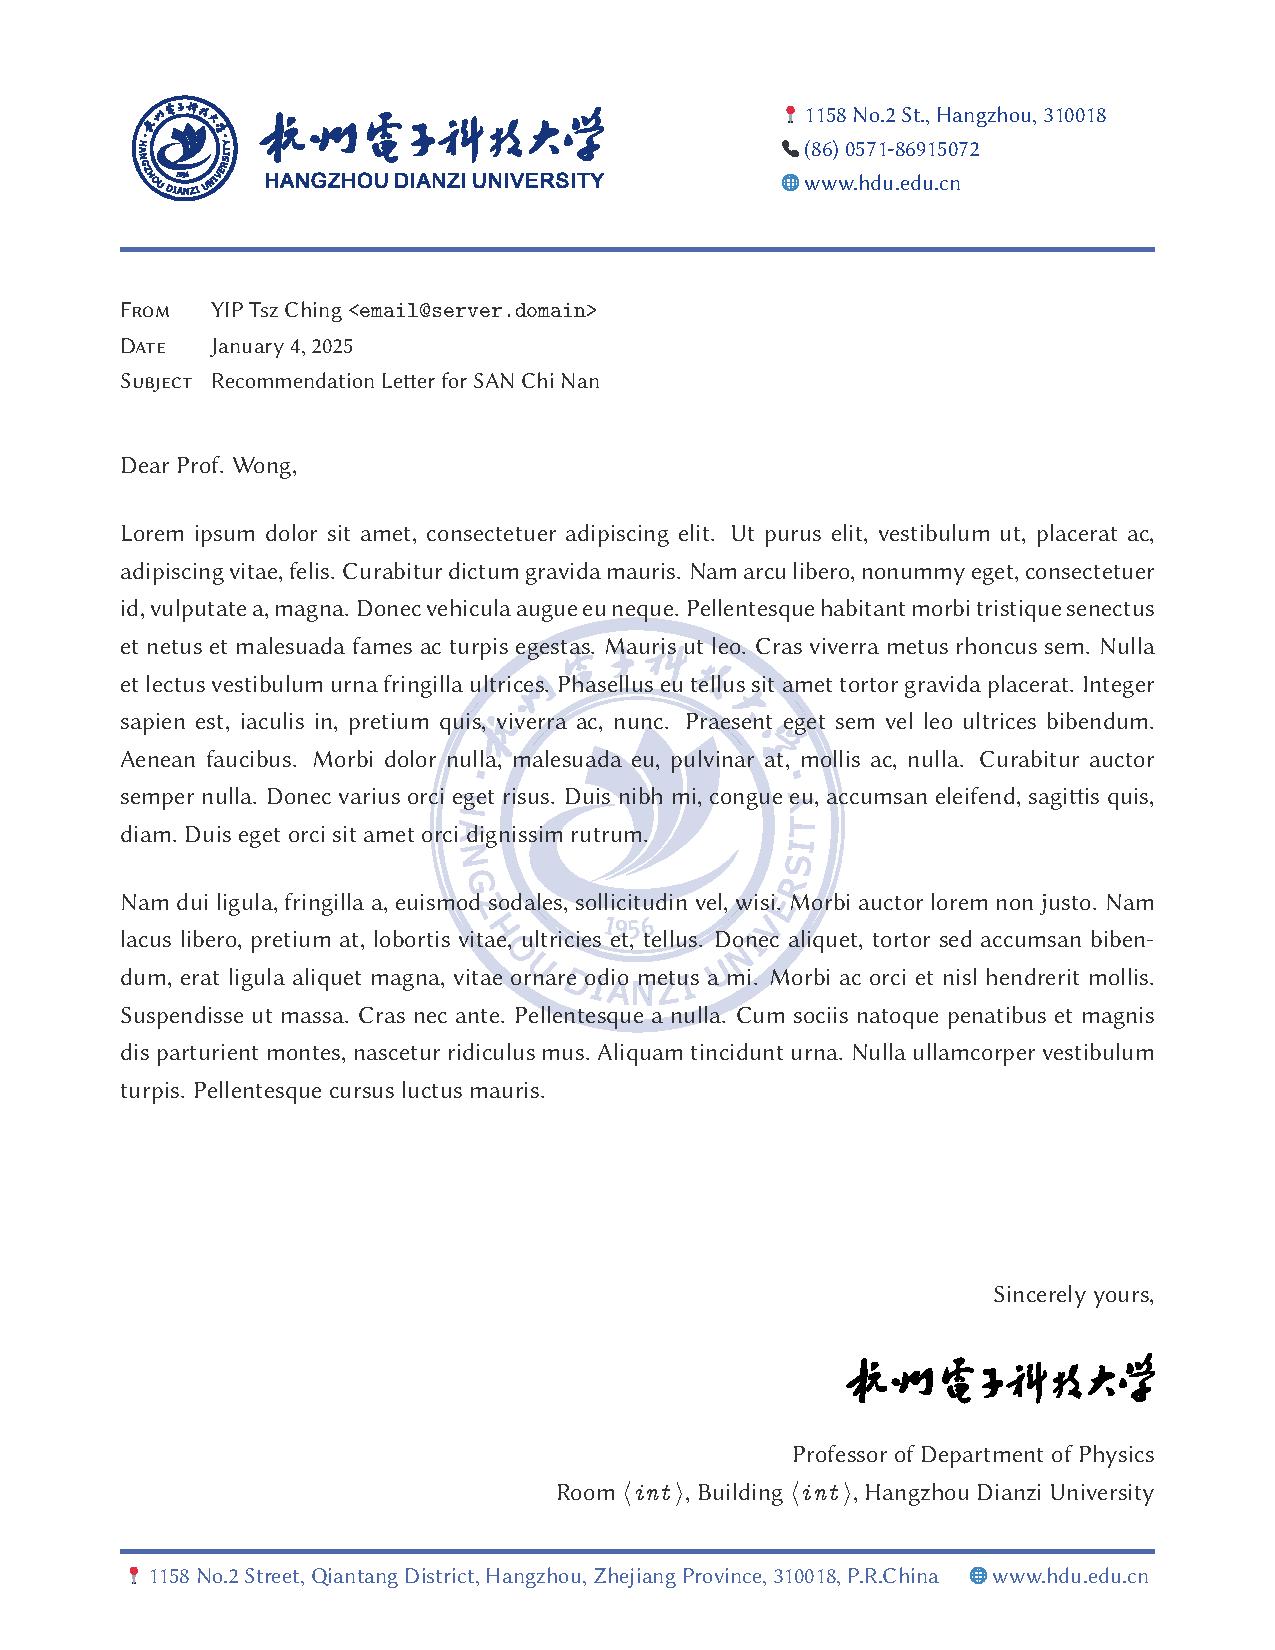
\includepdf[pages = -, nup = 1x2, angle = -90, frame, linktodoc, scale = 0.96, delta = 0in .25in]
  {/Users/myhsia/Documents/GitHub/hduthesis/example/hduthesis-stationery}

\subsection{Beamer 主题}

本模板中存在独立的 Beamer 主题 \cls{hdu},用于生成杭州电子科技大学风格的 Beamer 幻灯片. 由于本主题为杭州电子科技大学专属,所以该主题暂不开放更改主题色杭电蓝和Logo.

\begin{center}
  \frame{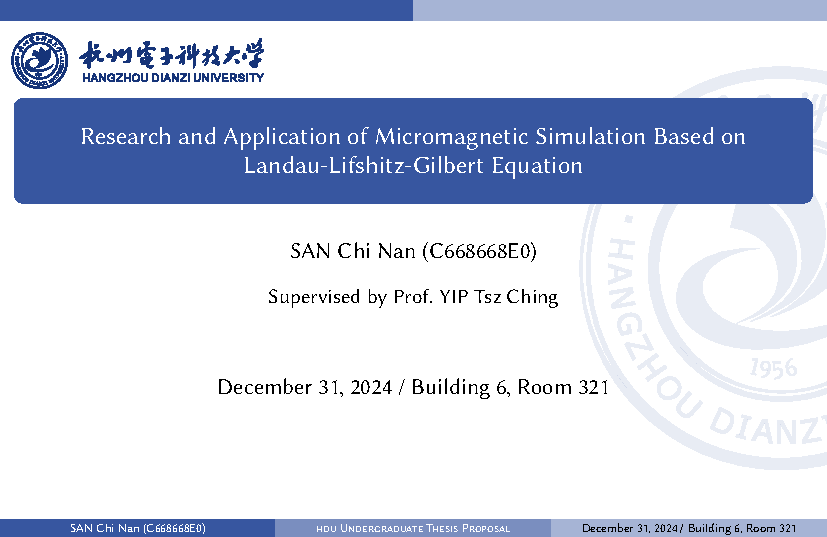
\includegraphics[width = .9\linewidth, page = 1]{/Users/myhsia/Documents/GitHub/hduthesis/example/hduthesis-beamer.pdf}}
  \par
  \frame{\includegraphics[width = .9\linewidth, page = 2]{/Users/myhsia/Documents/GitHub/hduthesis/example/hduthesis-beamer.pdf}}
\end{center}